\documentclass[11pt,openany]{article}

\usepackage{mathtools, commath}
% Packages for formatting
\usepackage[margin=1in]{geometry}
\usepackage{fancyhdr}
\usepackage{enumerate}
\usepackage{graphicx}
\usepackage{kotex}
\usepackage{amsmath}
\usepackage{amsthm}
\usepackage[dvipsnames,table]{xcolor}
\usepackage{amssymb, amsfonts}

\usepackage{arydshln} % Include this package
% Fonts
\usepackage[T1]{fontenc}
\usepackage[utf8]{inputenc}
\usepackage{newpxtext,newpxmath}
\usepackage{sectsty}

% Define colors
\definecolor{TealBlue1}{HTML}{0077c2}
\definecolor{TealBlue2}{HTML}{00a5e6}
\definecolor{TealBlue3}{HTML}{b3e0ff}
\definecolor{TealBlue4}{HTML}{00293c}
\definecolor{TealBlue5}{HTML}{e6f7ff}

\definecolor{thmcolor}{RGB}{231, 76, 60}
\definecolor{defcolor}{RGB}{52, 152, 219}
\definecolor{lemcolor}{RGB}{155, 89, 182}
\definecolor{corcolor}{RGB}{46, 204, 113}
\definecolor{procolor}{RGB}{241, 196, 15}

\usepackage{color,soul}
\usepackage{soul}
\newcommand{\mathcolorbox}[2]{\colorbox{#1}{$\displaystyle #2$}}
\usepackage{cancel}
\newcommand\crossout[3][black]{\renewcommand\CancelColor{\color{#1}}\cancelto{#2}{#3}}
\newcommand\ncrossout[2][black]{\renewcommand\CancelColor{\color{#1}}\cancel{#2}}

\usepackage{hyperref}
\usepackage{booktabs}

% Chapter formatting
\definecolor{titleTealBlue}{RGB}{0,53,128}
\usepackage{titlesec}
\titleformat{\section}
{\normalfont\sffamily\Large\bfseries\color{titleTealBlue!100!gray}}{\thesection}{1em}{}
\titleformat{\subsection}
{\normalfont\sffamily\large\bfseries\color{titleTealBlue!50!gray}}{\thesubsection}{1em}{}

%Tcolorbox
\usepackage[most]{tcolorbox}
\usepackage{multirow}
\usepackage{multicol}

\usepackage[linesnumbered,ruled]{algorithm2e}
\usepackage{algpseudocode}
\usepackage{setspace}
\SetKwComment{Comment}{/* }{ */}
\SetKwProg{Fn}{Function}{:}{end}
\SetKw{End}{end}
\SetKw{DownTo}{downto}

% Define a new environment for algorithms without line numbers
\newenvironment{algorithm2}[1][]{
	% Save the current state of the algorithm counter
	\newcounter{tempCounter}
	\setcounter{tempCounter}{\value{algocf}}
	% redefine the algorithm numbering (remove prefix)
	\renewcommand{\thealgocf}{}
	\begin{algorithm}
	}{
	\end{algorithm}
	% Restore the algorithm counter state
	\setcounter{algocf}{\value{tempCounter}}
}

\usepackage{adjustbox}
% Header and footer formatting
\pagestyle{fancy}
\fancyhead{}
\fancyhf{}
\rhead{\textcolor{TealBlue2}{\large\textbf{구체화에서 추상화에 이르는 대수학의 아름다움}}}%\rule{3cm}{0.4pt}}
\lhead{\textcolor{TealBlue2}{\large\textbf{수학의 즐거움}}}
% Define footer
\newcommand{\footer}[1]{
\begin{flushright}
	\vspace{2em}
	\includegraphics[width=2.5cm]{school_logo.jpg} \\
	\vspace{1em}
	\textcolor{TealBlue2}{\small\textbf{#1}}
\end{flushright}
}
%\rfoot{\large Department of Information Security, Cryptogrphy and Mathematics, Kookmin Uni.\includegraphics[height=1.5cm]{school_logo.jpg}}
\fancyfoot{}
\fancyfoot[C]{-\thepage-}

\newcommand{\ie}{\textnormal{i.e.}}
\newcommand{\rsa}{\mathsf{RSA}}
\newcommand{\rsacrt}{\mathsf{RSA}\textendash\mathsf{CRT}}
\newcommand{\inv}[1]{#1^{-1}}

\usepackage{amsthm}
\newtheorem{axiom}{Axiom}[section]
\newtheorem{theorem}{Theorem}
\newtheorem*{theorem*}{Theorem}
\newtheorem{proposition}[theorem]{Proposition}
\newtheorem{corollary}{Corollary}[theorem]
\newtheorem*{corollary*}{Corollary}
\newtheorem{lemma}[theorem]{Lemma}
\newtheorem*{lemma*}{Lemma}

\theoremstyle{definition}
\newtheorem{definition}{Definition}
\newtheorem*{notation*}{Notation}
\newtheorem*{definition*}{Definition}
\newtheorem*{note}{Note}
\newtheorem{remark}{Remark}
\newtheorem{example}{Example}
\newtheorem*{example*}{Example}
\newtheorem{exercise}{Exercise}[section]

%New Command
%\newcommand{\set}[1]{\left\{#1\right\}}
\newcommand{\N}{\mathbb{N}}
\newcommand{\Z}{\mathbb{Z}}
\newcommand{\Q}{\mathbb{Q}}
\newcommand{\R}{\mathbb{R}}
\newcommand{\C}{\mathbb{C}}
\newcommand{\F}{\mathbb{F}}
\newcommand{\nbhd}{\mathcal{N}}
\newcommand{\Log}{\operatorname{Log}}
\newcommand{\Arg}{\operatorname{Arg}}
\newcommand{\pv}{\operatorname{P.V.}}

\newcommand{\of}[1]{\left( #1 \right)} 
%\newcommand{\abs}[1]{\left\lvert #1 \right\rvert}
%\newcommand{\norm}[1]{\left\| #1 \right\|}

\newcommand{\sol}{\textcolor{magenta}{\bf Sol}}
\newcommand{\conjugate}[1]{\overline{#1}}

\newcommand{\res}{\operatorname{res}}
\DeclareMathOperator*{\Res}{\operatorname{Res}}

\renewcommand{\Re}{\operatorname{Re}}
\renewcommand{\Im}{\operatorname{Im}}

\newcommand{\cyclic}[1]{\langle #1 \rangle}
\newcommand{\uniform}{\overset{\$}{\leftarrow}}

\usepackage{caption}
%Tikzpicture
\usepackage{tikz}
\usepackage{tikz-3dplot}
\usepackage{tikz-cd}
\usetikzlibrary{
3d, % For 3D drawing
angles,
arrows,
arrows.meta,
backgrounds,
bending,
calc,
decorations.pathmorphing,
decorations.pathreplacing,
decorations.markings,
fit,
matrix,
patterns,
patterns.meta,
positioning,
quotes,
shadows,
shapes,
shapes.geometric
}

\newcommand{\arrowboth}[1][]{\arrow[#1, bend left=15, myarrow]\arrow[bend left=15, myarrow, from=#1]}

\setstretch{1.25}
\begin{document}
\pagenumbering{arabic}
\begin{center}
\huge\textbf{Quadratic Formula}\\
\vspace{0.5em}
%	\Large\quad{대수학의 아름다움 서브-스터디}\\
\vspace{0.5em}
\normalsize{\today}\\
\end{center}
\[
x^2-1=0\quad\iff\quad (x-1)(x+1)=0
\]
\begin{itemize}
	\item $a_1=0$, $a_0=-1$.
	\item $z=1$ and $z'=-1$
\end{itemize}
\begin{center}
\begin{minipage}{.48\textwidth}\centering
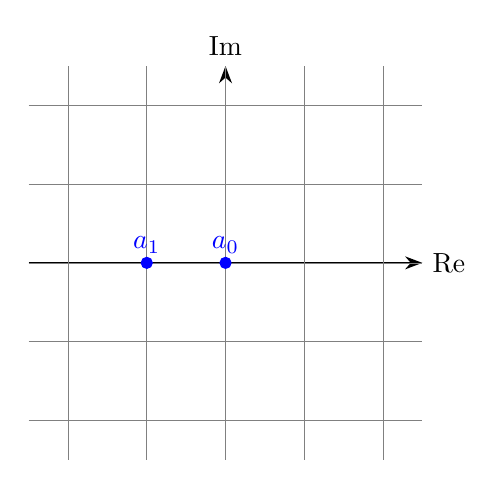
\begin{tikzpicture}[>=Stealth]
	% Axes
	\draw[->, line width=.25mm] (-2.5,0) -- (2.5,0) node[right] {$\Re$};
	\draw[->, line width=.25mm] (0,-2.5) -- (0,2.5) node[above] {$\Im$};
	
	% Grid
	\draw[very thin,color=gray] (-2.5,-2.5) grid (2.5,2.5);
	
	% Points for roots
	\filldraw[blue] (0,0) circle (2pt) node[anchor=south] {$a_0$};
	\filldraw[blue] (-1,0) circle (2pt) node[anchor=south] {$a_1$};
\end{tikzpicture}
\end{minipage}
\begin{minipage}{.48\textwidth}\centering
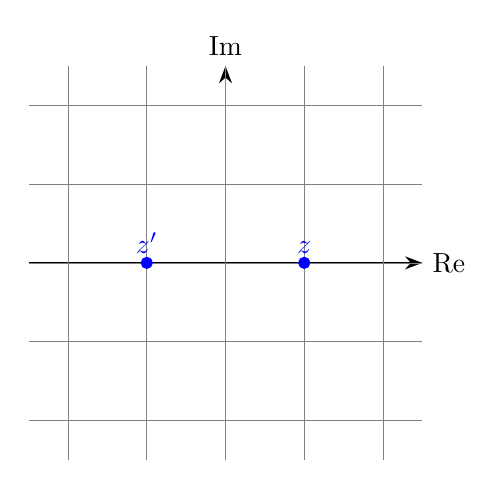
\begin{tikzpicture}[>=Stealth]
	% Axes
	\draw[->, line width=.25mm] (-2.5,0) -- (2.5,0) node[right] {$\Re$};
	\draw[->, line width=.25mm] (0,-2.5) -- (0,2.5) node[above] {$\Im$};
	
	% Grid
	\draw[very thin,color=gray] (-2.5,-2.5) grid (2.5,2.5);
	
	% Points for roots
	\filldraw[blue] (1,0) circle (2pt) node[anchor=south] {$z$};
	\filldraw[blue] (-1,0) circle (2pt) node[anchor=south] {$z'$};
\end{tikzpicture}
\end{minipage}
\end{center}
\begin{tikzpicture}
	% Axes
	\draw[->] (-2.5,0) -- (2.5,0) node[anchor=north west] {Re};
	\draw[->] (0,-2.5) -- (0,2.5) node[anchor=south east] {Im};
	
	% Unit circle
	\draw[gray] (0,0) circle (2);
	
	% Parameter theta
	\def\theta{45} % theta in degrees
	
	% Calculate the roots
	\coordinate (A) at ({2*cos(\theta)},{2*sin(\theta)});
	\coordinate (B) at ({2*cos(\theta+180)},{2*sin(\theta+180)});
	
	% Draw the roots
	\filldraw[blue] (A) circle (2pt) node[anchor=south] {$e^{i\theta}$};
	\filldraw[blue] (B) circle (2pt) node[anchor=north] {$e^{i(\theta + \pi)}$};
	
	% Labels
	\node at (2.5, 2.2) [anchor=south west] {Complex Plane};
\end{tikzpicture}

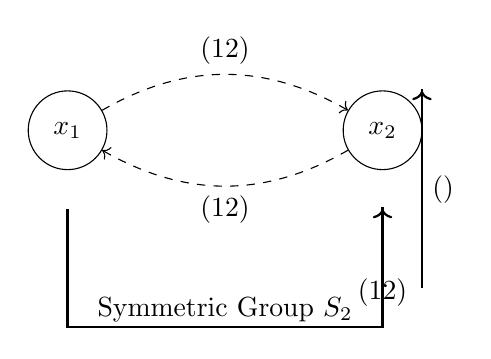
\begin{tikzpicture}
	
	% Nodes representing the roots
	\node[draw, circle, minimum size=1cm] (x1) at (0,0) {$x_1$};
	\node[draw, circle, minimum size=1cm] (x2) at (4,0) {$x_2$};
	
	% Identity permutation arrow
	\draw[->, thick] (0,-1) -- (0,-2.5) -- (4,-2.5) -- (4,-1) node[midway,below] {$(12)$} -- (4,-1);
	
	% Transposition arrow
	\draw[->, thick] (4.5,-2) -- (4.5,0.5) node[midway,right] {$()$} -- (4.5,0.5);
	
	% Label for S_2
	\node at (2,-2) [anchor=north] {Symmetric Group $S_2$};
	
	% Arrows showing root swapping
	\draw[->, dashed] (x1) to [bend left] node[midway,above] {$(12)$} (x2);
	\draw[->, dashed] (x2) to [bend left] node[midway,below] {$(12)$} (x1);
	
\end{tikzpicture}
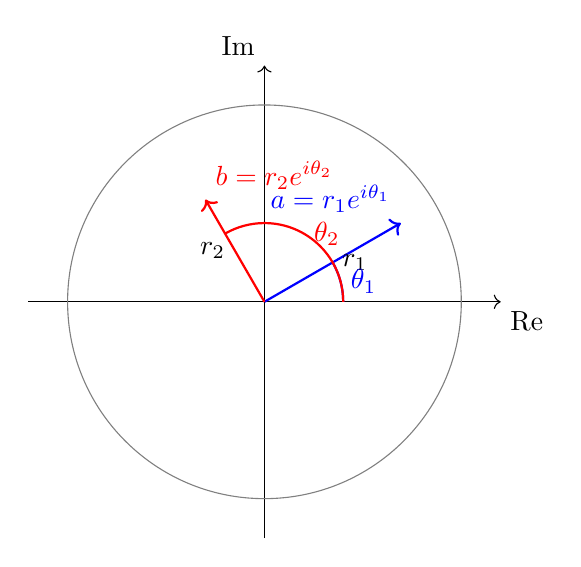
\begin{tikzpicture}
	
	% Draw the complex plane
	\draw[->] (-3,0) -- (3,0) node[anchor=north west] {Re};
	\draw[->] (0,-3) -- (0,3) node[anchor=south east] {Im};
	
	% Draw the unit circle
	\draw[gray] (0,0) circle (2.5);
	
	% Draw a
	\draw[->, thick, blue] (0,0) -- ({2*cos(30)}, {2*sin(30)}) node[anchor=south east] {$a = r_1 e^{i\theta_1}$};
	\node at ({2*cos(30)/2}, {2*sin(30)/2}) [anchor=west] {$r_1$};
	
	% Draw b
	\draw[->, thick, red] (0,0) -- ({1.5*cos(120)}, {1.5*sin(120)}) node[anchor=south west] {$b = r_2 e^{i\theta_2}$};
	\node at ({1.5*cos(120)/2}, {1.5*sin(120)/2}) [anchor=east] {$r_2$};
	
	% Draw angle for a
	\draw[thick,blue] (1,0) arc[start angle=0, end angle=30, radius=1] node[midway,right] {$\theta_1$};
	
	% Draw angle for b
	\draw[thick,red] (1,0) arc[start angle=0, end angle=120, radius=1] node[midway,right] {$\theta_2$};
	
\end{tikzpicture}

\begin{tikzpicture}
	
	% Draw the complex plane
	\draw[->] (-2.5,0) -- (2.5,0) node[anchor=north west] {Re};
	\draw[->] (0,-2.5) -- (0,2.5) node[anchor=south east] {Im};
	
	% Draw the unit circle
	\draw[gray] (0,0) circle (2);
	
	% Plot the roots for (x-1)(x+1) = 0
	\filldraw[blue] (2,0) circle (2pt) node[anchor=south] {$1$};
	\filldraw[blue] (-2,0) circle (2pt) node[anchor=south] {$-1$};
	
	% Plot the root for (x-1)(x+1)(x-i) = 0
	\filldraw[red] (0,2) circle (2pt) node[anchor=west] {$i$};
	
	% Label angles for cubic roots
	\node at (2.3, 0.3) {$\theta = 0$};
	\node at (-2.5, 0.3) {$\theta = \pi$};
	\node at (0.3, 2.3) {$\theta = \frac{\pi}{2}$};
	
\end{tikzpicture}

\begin{center}
\begin{tikzpicture}[scale=1.25]
	% 1. Quadratic Coefficient Plane
	\node at (-7,1.5) [anchor=west] {\textbf{Coefficients of}\ $x^2-1$};
	
	% Draw the complex plane for coefficients
	\draw[->] (-7,4) -- (-3,4) node[right] {Re};
	\draw[->] (-5,2) -- (-5,6) node[above] {Im};
	
	% Plot the coefficients
	\filldraw[blue] (-5,4) circle (2pt) node[anchor=south] {$0$};
	\filldraw[blue] (-6,4) circle (2pt) node[anchor=south] {$-1$};
	
	% Unit circle
	\draw[gray] (-5,4) circle (1);
	
	% 2. Quadratic Root Plane
	\node at (-1,1.75) [] {$\xleftarrow[]{\text{easy}}$};
	\node at (-1,1.25) [] {$\xrightarrow[\text{difficult}]{}$};
	\node at (1,1.5) [anchor=west] {\textbf{Roots of}\ $(x+1)(x-1)$};
	
	% Draw the complex plane for roots
	\draw[->] (1,4) -- (5,4) node[right] {Re};
	\draw[->] (3,2) -- (3,6) node[above] {Im};
	
	% Plot the roots
	\filldraw[red] (4,4) circle (2pt) node[anchor=south] {$1$};
	\filldraw[red] (2,4) circle (2pt) node[anchor=south] {$-1$};
	
	% Unit circle
	\draw[gray] (3,4) circle (1);
	
	% 3. Cubic Coefficient Plane
	\node at (-7,-4.5) [anchor=west] {\textbf{Coefficients}\ $x^3-ix^2-x+i$};
	
	% Draw the complex plane for coefficients
	\draw[->] (-7,-2) -- (-3,-2) node[right] {Re};
	\draw[->] (-5,-4) -- (-5,0) node[above] {Im};
	
	% Plot the coefficients
	\filldraw[blue] (-5,-1) circle (2pt) node[anchor=west] {$i$};
	\filldraw[blue] (-6,-2) circle (2pt) node[anchor=south] {$-1$};
	\filldraw[blue] (-5,-3) circle (2pt) node[anchor=west] {$-i$};
	
	% Unit circle
	\draw[gray] (-5,-2) circle (1);
	
	% 4. Cubic Root Plane
	\node at (-1,-4.25) [] {$\xleftarrow[]{\text{easy}}$};
	\node at (-1,-4.75) [] {$\xrightarrow[\text{difficult}]{}$};
	\node at (1,-4.5) [anchor=west] {\textbf{Roots of}\ $(x-1)(x+1)(x-i)$};
	
	% Draw the complex plane for roots
	\draw[->] (1,-2) -- (5,-2) node[right] {Re};
	\draw[->] (3,-4) -- (3,0) node[above] {Im};
	
	% Plot the roots
	\filldraw[red] (4,-2) circle (2pt) node[anchor=south] {$1$};
	\filldraw[red] (2,-2) circle (2pt) node[anchor=south] {$-1$};
	\filldraw[red] (3,-1) circle (2pt) node[anchor=west] {$i$};
	
	% Unit circle
	\draw[gray] (3,-2) circle (1);
\end{tikzpicture}
\end{center}
\newpage
\begin{center}
\begin{tikzpicture}[scale=1.25]
	% 1. Quadratic Coefficient Plane
	\node at (-7,1.5) [anchor=west] {\textbf{Coefficients of}\ $x^2-1$};
	
	% Draw the complex plane for coefficients
	\draw[->] (-7,4) -- (-3,4) node[right] {Re};
	\draw[->] (-5,2) -- (-5,6) node[above] {Im};
	
	% Plot the coefficients
	\filldraw[blue] (-5,4) circle (2pt) node[anchor=south] {$0$};
	\filldraw[blue] (-6,4) circle (2pt) node[anchor=south] {$-1$};
	
	% Unit circle
	\draw[gray] (-5,4) circle (1);
	
	% 2. Quadratic Root Plane
	\node at (1,1.5) [anchor=west] {\textbf{Roots of}\ $(x+1)(x-1)$};
	
	% Draw the complex plane for roots
	\draw[->] (1,4) -- (5,4) node[right] {Re};
	\draw[->] (3,2) -- (3,6) node[above] {Im};
	
	% Plot the roots
	\filldraw[red] (4,4) circle (2pt) node[anchor=south] {$1$};
	\filldraw[red] (2,4) circle (2pt) node[anchor=south] {$-1$};
	
	% Unit circle
	\draw[gray] (3,4) circle (1);
\end{tikzpicture}
\end{center}
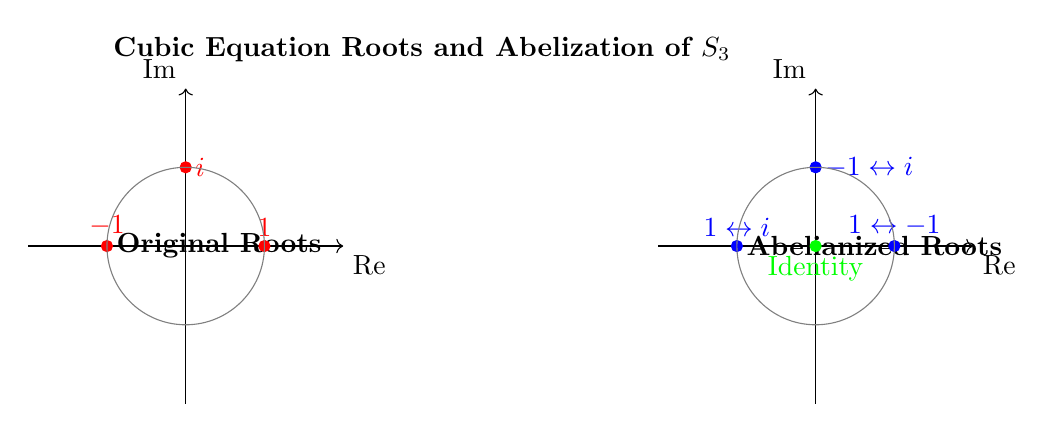
\begin{tikzpicture}
	
	% Title for the diagram
	\node at (0,4.5) {\textbf{Cubic Equation Roots and Abelization of \(S_3\)}};
	
	% 1. Original Root Plane
	\node at (-4,2) [anchor=west] {\textbf{Original Roots}};
	
	% Draw the complex plane for original roots
	\draw[->] (-5,2) -- (-1,2) node[anchor=north west] {Re};
	\draw[->] (-3,0) -- (-3,4) node[anchor=south east] {Im};
	
	% Plot the original roots
	\filldraw[red] (-2,2) circle (2pt) node[anchor=south] {$1$};
	\filldraw[red] (-4,2) circle (2pt) node[anchor=south] {$-1$};
	\filldraw[red] (-3,3) circle (2pt) node[anchor=west] {$i$};
	
	% Unit circle
	\draw[gray] (-3,2) circle (1);
	
	% 2. Abelianized Root Plane
	\node at (4,2) [anchor=west] {\textbf{Abelianized Roots}};
	
	% Draw the complex plane for Abelianized roots
	\draw[->] (3,2) -- (7,2) node[anchor=north west] {Re};
	\draw[->] (5,0) -- (5,4) node[anchor=south east] {Im};
	
	% Plot the Abelianized roots (transpositions and identity)
	\filldraw[blue] (6,2) circle (2pt) node[anchor=south] {$1 \leftrightarrow -1$};
	\filldraw[blue] (4,2) circle (2pt) node[anchor=south] {$1 \leftrightarrow i$};
	\filldraw[blue] (5,3) circle (2pt) node[anchor=west] {$-1 \leftrightarrow i$};
	
	% Unit circle
	\draw[gray] (5,2) circle (1);
	
	% Identity element
	\filldraw[green] (5,2) circle (2pt) node[anchor=north] {Identity};
	
\end{tikzpicture}

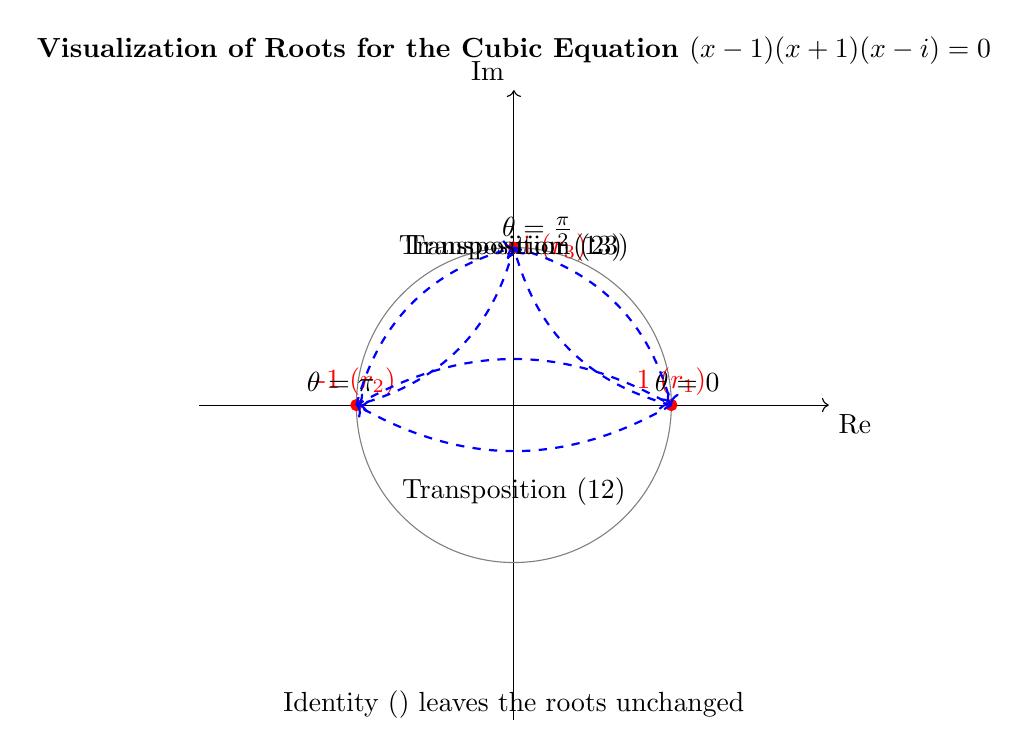
\begin{tikzpicture}
	
	% Title for the diagram
	\node at (0,4.5) {\textbf{Visualization of Roots for the Cubic Equation \((x - 1)(x + 1)(x - i) = 0\)}};
	
	% Draw the complex plane
	\draw[->] (-4,0) -- (4,0) node[anchor=north west] {Re};
	\draw[->] (0,-4) -- (0,4) node[anchor=south east] {Im};
	
	% Draw the unit circle
	\draw[gray] (0,0) circle (2);
	
	% Plot the original roots
	\filldraw[red] (2,0) circle (2pt) node[anchor=south] {1 ($r_1$)};
	\filldraw[red] (-2,0) circle (2pt) node[anchor=south] {-1 ($r_2$)};
	\filldraw[red] (0,2) circle (2pt) node[anchor=west] {i ($r_3$)};
	
	% Label the roots on the unit circle
	\node at (2.2, 0.3) {$\theta = 0$};
	\node at (-2.2, 0.3) {$\theta = \pi$};
	\node at (0.3, 2.2) {$\theta = \frac{\pi}{2}$};
	
	% Draw arrows for S3 Abelianized actions
	% Transposition (12)
	\draw[->, thick, blue, dashed] (2,0) to [bend left=30] (-2,0);
	\draw[->, thick, blue, dashed] (-2,0) to [bend left=30] (2,0);
	\node at (0, -0.8) [anchor=north] {Transposition \((12)\)};
	
	% Transposition (13)
	\draw[->, thick, blue, dashed] (2,0) to [bend left=30] (0,2);
	\draw[->, thick, blue, dashed] (0,2) to [bend left=30] (2,0);
	\node at (1.5, 1.7) [anchor=south east] {Transposition \((13)\)};
	
	% Transposition (23)
	\draw[->, thick, blue, dashed] (-2,0) to [bend left=30] (0,2);
	\draw[->, thick, blue, dashed] (0,2) to [bend left=30] (-2,0);
	\node at (-1.5, 1.7) [anchor=south west] {Transposition \((23)\)};
	
	% Identity element
	\node at (0, -3.5) [anchor=north] {Identity \(()\) leaves the roots unchanged};
	
\end{tikzpicture}
\newpage

\section*{Product of Ideals}
\subsection*{Product of Ideals (without finite sums)}
Given two ideals $I$ and $J$ in a ring $R$, the product $IJ$ without finite sums is defined as: \[
IJ\triangleq\set{ab:a\in I,b\in J}.
\]
\paragraph{[Example in $\Z$]}

Consider $I=2\Z$ and $J=3\Z$ in $\Z$: \begin{align*}
2\Z&=\set{2n:n\in\Z},\\
3\Z&=\set{3m:m\in\Z}.
\end{align*} By definition, \[
IJ=\set{2n\cdot 3m:n,m\in\Z}=\set{6nm:n,m\in\Z}.
\] Consider two general elements $6n_1m_1$ and $6n_2m_2$ in $IJ$.
Their sum is \[
6n_1m_2+6n_2m_2=6(n_1m_1+n_2m_2)=6\sum_{k=1}^{2}n_km_k\mathcolorbox{-red}{\overset{?}{\in}IJ=\set{6nm:n,m\in\Z}}.
\] Without finite sums, we only have products $6ab$.
\subsection*{Product of Ideals (with finite sums)}
\[
IJ\triangleq\set{\sum_{k=1}^ta_kb_k:a_k\in I,b_k\in J,t\in\N}.
\] Consider $x=\sum_{k=1}^s6a_kb_k$ and $y=\sum_{k=1}^t6a_kb_k$. Then \begin{align*}
x+y=\sum_{k=1}^s6a_kb_k+\sum_{l=1}^t6a_lb_l&=6\left(\sum_{k=1}^sa_kb_k+\sum_{k=1}^ta_kb_k\right)
\\&=6\sum_{k=1}^{s+t}a_kb_k
\end{align*}
\newpage
\paragraph{[Example in $\C[x]$]}
\subsection*{Product of Ideals (without finite sums)}
Consider $I=(x)$ and $J=(x^2)$ in $\C[x]$: \begin{align*}
(x)&=\set{x\cdot p(x):p(x)\in\C[x]},\\
(x^2)&=\set{x^2\cdot q(x):q\in\C[x]}.
\end{align*} By definition, \[
IJ=\set{x\cdot p(x)\cdot x^2\cdot q(x):p(x),q(x)\in\C[x]}=\set{x^3p(x)q(x):p(x),q(x)\in\C[x]}.
\] Consider two general elements $x^3p_1(x)q_1(x)$ and $x^3p_2(x)q_2(x)$ in $IJ$.
Their sum is \[
x^3p_1(x)q_1(x)+x^3p_2(x)q_2(x)=x^3(p_1(x)q_1(x)+p_2(x)q_2(x))=x^3\sum_{i=1}^2p_i(x)q_i(x).
\]
\subsection*{Product of Ideals (with finite sums)}
\[
IJ\triangleq\set{\sum_{k=1}^ta_kb_k:a_k\in I,b_k\in J,t\in\N}.
\] Consider $x=\sum_{k=1}^s6a_kb_k$ and $y=\sum_{k=1}^t6a_kb_k$. Then \begin{align*}
x+y=\sum_{k=1}^s6a_kb_k+\sum_{l=1}^t6a_lb_l&=6\left(\sum_{k=1}^sa_kb_k+\sum_{k=1}^ta_kb_k\right)
\\&=6\sum_{k=1}^{s+t}a_kb_k
\end{align*}

\newpage
\paragraph{[Example in $\Z[x]$]}
Consider $I=(2,x)$ and $J=(3,x^2)$ in $\Z[x]$: \begin{align*}
(2,x)&=\set{2f(x)+xg(x):f,g\in\Z[x]},\\
(3,x^2)&=\set{3h(x)+x^2k(x):h,k\in\C[x]}.
\end{align*} Let \[
IJ\triangleq\set{(2f+xg)(3h+x^2k):f,g,h,k\in\Z[x]}.
\] Consider \begin{align*}
x_1&=(2+x)(3+x^2)\in IJ,\\
x_2&=(2x+x^3)(3+x^2)\in IJ.
\end{align*} Then \begin{align*}
x_1&=(2+x)(3+x^2)=6+2x^2+3x+x^3,\\
x_2&=6x+2x^3+3x^3+x^5=6x+5x^3+x^5.
\end{align*}

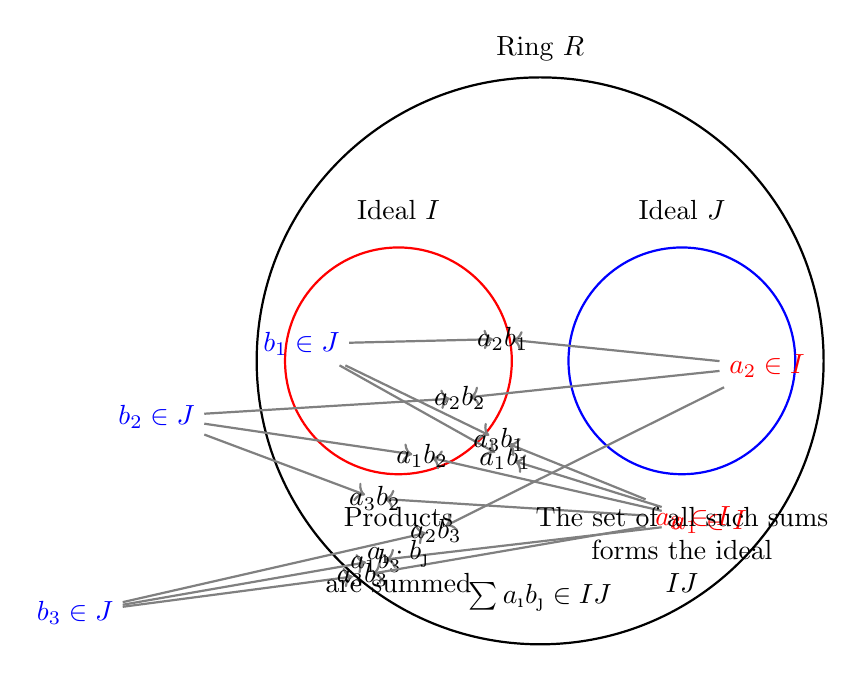
\begin{tikzpicture}[scale=1.2]

% Draw the ring
\draw[thick] (0, 0) circle (3cm);
\node at (0, 3.3) {Ring $R$};

% Draw ideal I
\draw[thick, red] (-1.5, 0) circle (1.2cm);
\node at (-1.5, 1.6) {Ideal $I$};

% Draw ideal J
\draw[thick, blue] (1.5, 0) circle (1.2cm);
\node at (1.5, 1.6) {Ideal $J$};

% Label elements in I
\foreach \i in {1,2,3}
{
	\node[red] (I\i) at ($(rand*2-1,rand*2-1)+(3,0)$) {$a_{\i} \in I$};
}

% Label elements in J
\foreach \j in {1,2,3}
{
	\node[blue] (J\j) at ($(rand*2-1,rand*2-1)-(3,0)$) {$b_{\j} \in J$};
}

% Draw the product of elements and their sum
\foreach \i in {1,2,3}
{
	\foreach \j in {1,2,3}
	{
		\node (P\i\j) at ($(I\i)!0.5!(J\j)+(rand*0.5-0.25,rand*0.5-0.25)$) {};
		\draw[thick, ->, gray] (I\i) -- (P\i\j);
		\draw[thick, ->, gray] (J\j) -- (P\i\j);
		\node[black] at (P\i\j) {$a_{\i} b_{\j}$};
	}
}

% Summation
\node at (0, -2.5) {$\sum a_{\i} b_{\j} \in IJ$};

% Additional labels
\node[align=center] at (-1.5, -2) {Products \\ $a_{\i} \cdot b_{\j}$ \\ are summed};
\node[align=center] at (1.5, -2) {The set of all such sums \\ forms the ideal \\ $IJ$};

\end{tikzpicture}
\newpage
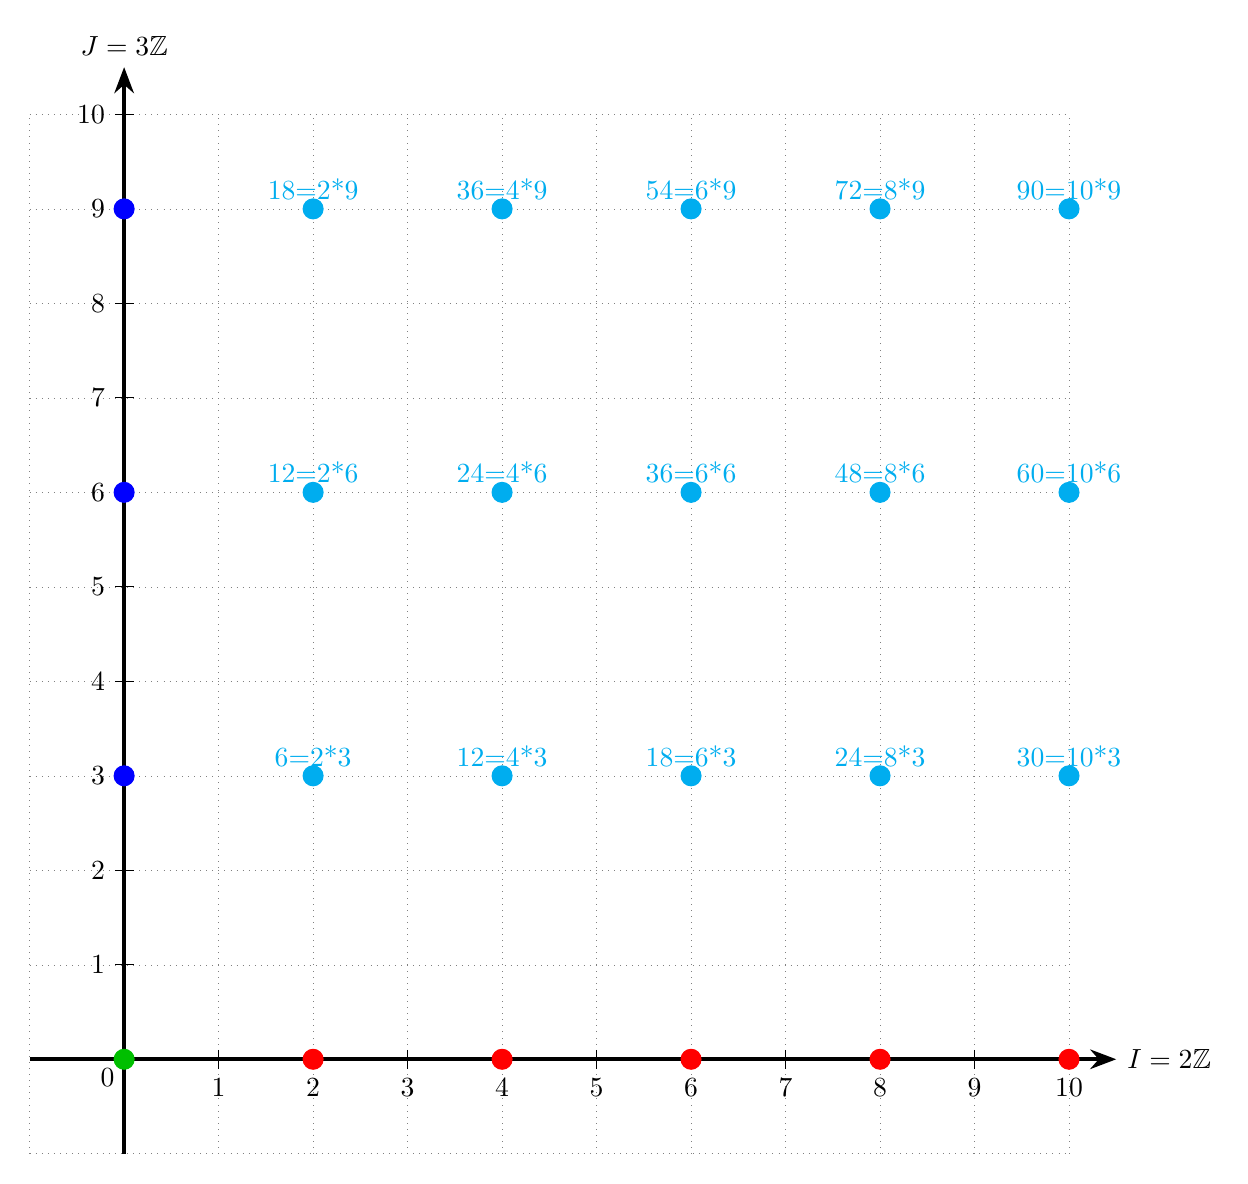
\begin{tikzpicture}[scale=1.2, every node/.style={scale=1.0}]

% Grid
\draw[step=1cm, dotted, gray, very thin] (-1, -1) grid (10, 10);

% Axes
\draw[-Stealth, thick, line width=.5mm] (-1,0) -- (10.5,0) node[right] {$I = 2\Z$};
\draw[-Stealth, thick, line width=.5mm] (0,-1) -- (0,10.5) node[above] {$J = 3\Z$};

%Take Coordinates
\foreach \i in {1,2,...,10}
\draw[] (\i,.1)--(\i,-.1) node[below] {$\i$};%x-axis
\foreach \i in {1,2,...,10}
\draw[] (.1,\i)--(-.1,\i) node[left] {$\i$};%y-axis

\node[below left] at (0,0) {$0$};
\filldraw[green!75!black] (0,0) circle (3pt);

% Points for Ideal (2)
\foreach \x in {2,4,...,10}
\filldraw[red] (\x,0) circle (3pt);

% Points for Ideal (3)
\foreach \y in {3,6,9}
\filldraw[blue] (0,\y) circle (3pt);

\foreach \x in {2,4,...,10} {
	\foreach \y in {3,6,9} {
		\pgfmathtruncatemacro{\result}{\x * \y}
		\filldraw[cyan] (\x,\y) circle (3pt) node[above] {\result=\x*\y};
	}
}

%		
%		% Points for Product Ideal (6)
%		\foreach \x in {0,1,2,3,4,5}
%		\foreach \y in {0,1,2,3,4,5}
%		\ifnum \numexpr \x*\y = \numexpr \x*\y/6*6
%		\filldraw[black] (\x,\y) circle (2pt);
%		\fi
%		
%		% Labels
%		\node[red, below] at (2, 0) {$2$};
%		\node[red, below] at (4, 0) {$4$};
%		
%		\node[blue, left] at (0, 3) {$3$};
%		\node[blue, left] at (0, 6) {$6$};
%		
%		\node[black, right] at (1, 6) {$6$};
%		\node[black, right] at (2, 3) {$6$};
%		\node[black, right] at (3, 2) {$6$};
%		\node[black, right] at (6, 1) {$6$};
%		
%		\node[above] at (2, 2) {$IJ = (6)$};
\end{tikzpicture}

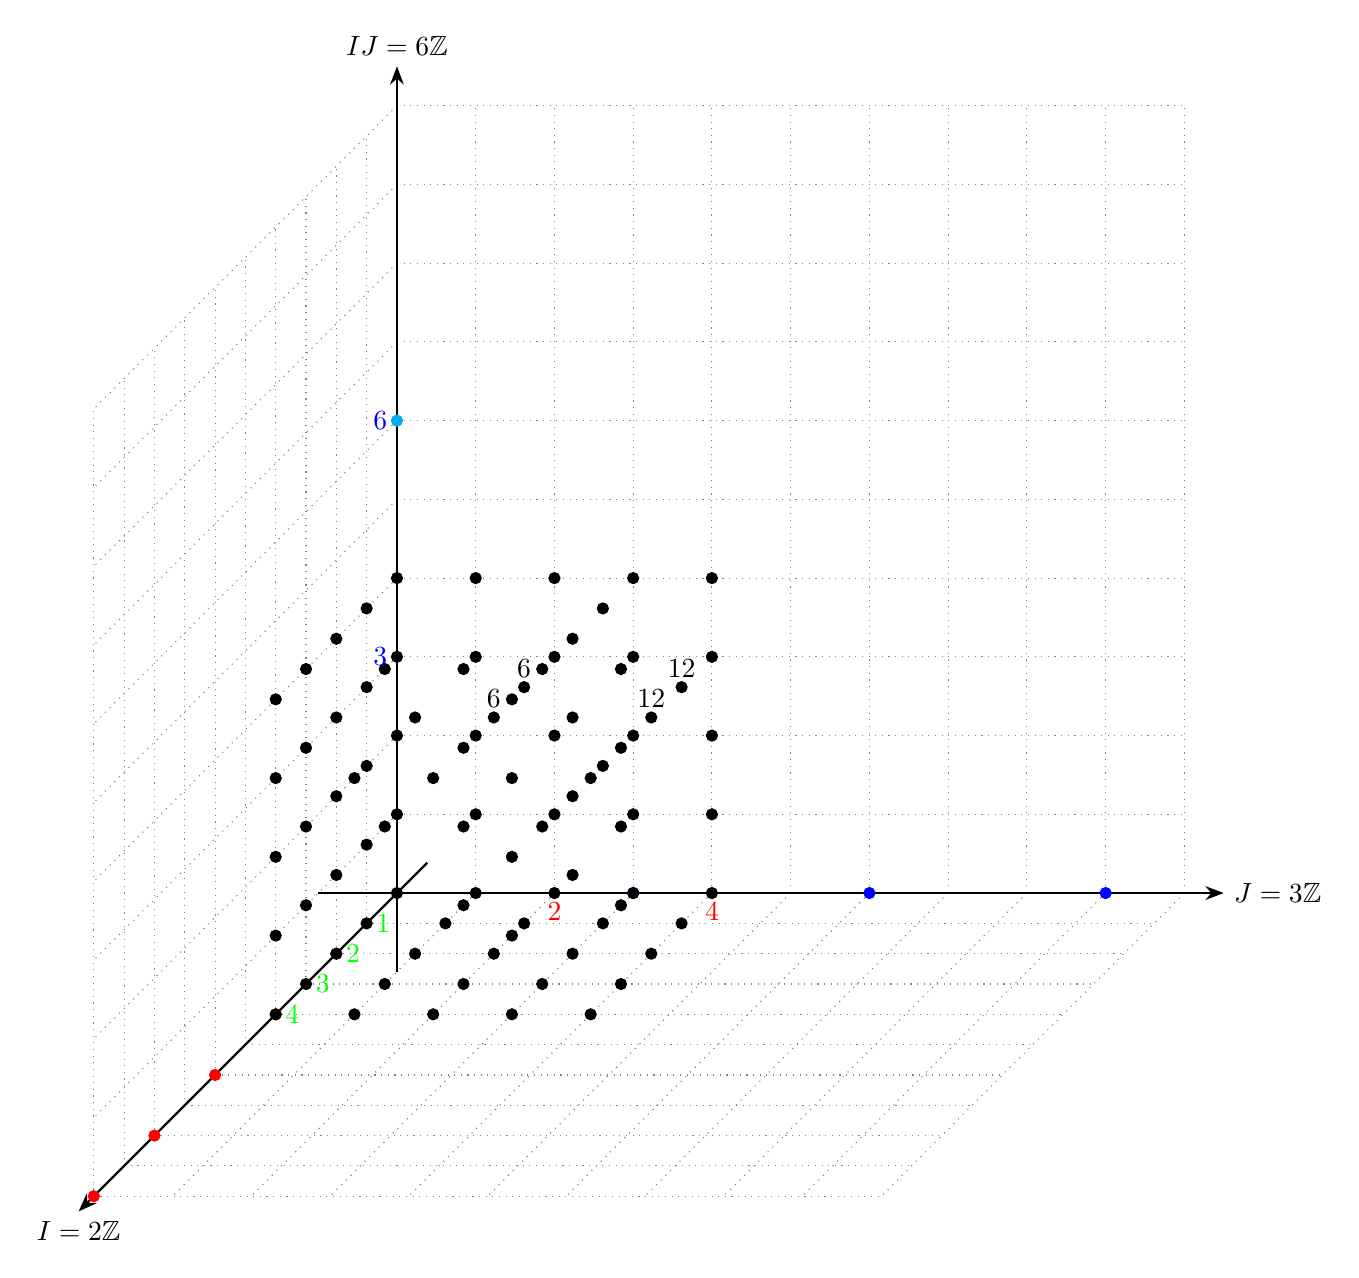
\begin{tikzpicture}[scale=1, every node/.style={scale=1.0}]

% Define the size of the grid
\def\xmax{10}
\def\ymax{10}
\def\zmax{10}

% Draw the 3D grid
%		\foreach \x in {-1,...,\xmax}
%		{
	%			\foreach \y in {-1,...,\ymax}
	%			{
		%				\foreach \z in {-1,...,\zmax}
		%				{
			%					\filldraw[gray,opacity=0.5] (\x,\y,\z) circle (1pt);
			%				}
		%			}
	%		}

% Grid
%		\draw[step=1cm, dotted, gray, very thin] (-1, -1, -1) grid (\xmax+2, \ymax+2, \zmax+2);

\foreach \i in {0,1,...,10} {
	\draw[step=1cm, dotted, gray] (0,\i,0) -- (0,\i,\xmax);
	\draw[step=1cm, dotted, gray] (\i,0,0) -- (\i,0,\xmax);
	\draw[step=1cm, dotted, gray] (0,\i,0) -- (\ymax,\i,0);
	\draw[step=1cm, dotted, gray] (0,0,\i) -- (\ymax,0,\i);
	\draw[step=1cm, dotted, gray] (\i,0,0) -- (\i,\zmax,0);
	\draw[step=1cm, dotted, gray] (0,0,\i) -- (0,\zmax,\i);
}

% Draw the axes
\draw[thick,-Stealth] (0,0,-1) -- (0,0,\xmax+.5) node[below] {$I = 2\Z$};
\draw[thick,-Stealth] (-1,0,0) -- (\ymax+.5,0,0) node[right] {$J = 3\Z$};
\draw[thick,-Stealth] (0,-1,0) -- (0,\zmax+.5,0) node[above] {$IJ = 6\Z$};

% Points for Ideal I (multiples of 2)
\foreach \x in {2,4,...,10} {
	\filldraw[red] (0,0,\x) circle (2pt);
}

% Points for Ideal J (multiples of 3)
\foreach \y in {3,6,...,9} {
	\filldraw[blue] (\y,0,0) circle (2pt);
}

% Points for Ideal K (multiples of 1)
\foreach \z in {6}
{
	\filldraw[cyan] (0,\z,0) circle (2pt);
}

% Points for Product Ideal IJ = (6)
\foreach \x in {0,1,2,3,4}
{
	\foreach \y in {0,1,2,3,4}
	{
		\foreach \z in {0,1,2,3,4}
		{
			\ifnum \numexpr \x*\y*\z = \numexpr \x*\y*\z/6*6
			\filldraw[black] (\x,\y,\z) circle (2pt);
			\fi
		}
	}
}

% Labels
\node[red, below] at (2, 0, 0) {$2$};
\node[red, below] at (4, 0, 0) {$4$};

\node[blue, left] at (0, 3, 0) {$3$};
\node[blue, left] at (0, 6, 0) {$6$};

\node[green, right] at (0, 0, 1) {$1$};
\node[green, right] at (0, 0, 2) {$2$};
\node[green, right] at (0, 0, 3) {$3$};
\node[green, right] at (0, 0, 4) {$4$};

\node[black, above] at (2, 3, 1) {$6$};
\node[black, above] at (2, 3, 2) {$6$};
\node[black, above] at (4, 3, 1) {$12$};
\node[black, above] at (4, 3, 2) {$12$};

\end{tikzpicture}

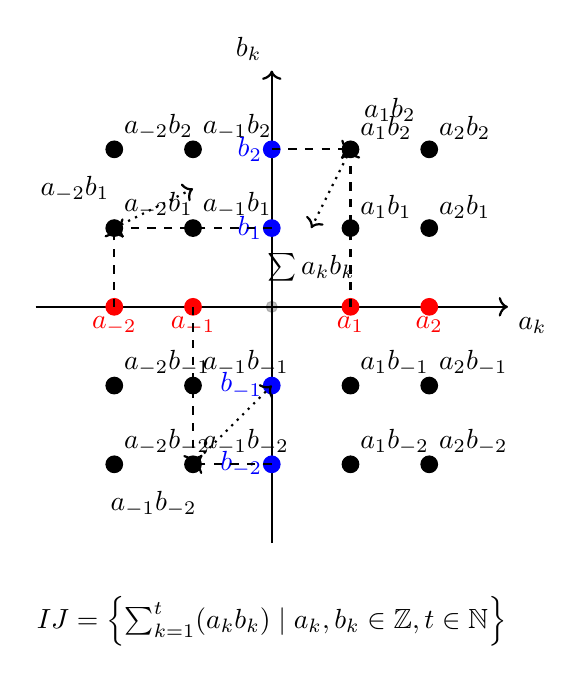
\begin{tikzpicture}[scale=1.0]

% Define the grid
\foreach \x in {-2, -1, 0, 1, 2}
{
	\foreach \y in {-2, -1, 0, 1, 2}
	{
		\filldraw[gray,opacity=0.5] (\x,\y) circle (2pt);
	}
}

% Axes
\draw[thick,->] (-3,0) -- (3,0) node[anchor=north west] {$a_k$};
\draw[thick,->] (0,-3) -- (0,3) node[anchor=south east] {$b_k$};

% Points for I = (a)
\foreach \x in {-2, -1, 1, 2}
{
	\filldraw[red] (\x,0) circle (3pt);
	\node[red, below] at (\x, 0) {$a_{\x}$};
}

% Points for J = (b)
\foreach \y in {-2, -1, 1, 2}
{
	\filldraw[blue] (0,\y) circle (3pt);
	\node[blue, left] at (0, \y) {$b_{\y}$};
}

% Points for Product a_i * b_j
\foreach \x in {-2, -1, 1, 2}
{
	\foreach \y in {-2, -1, 1, 2}
	{
		\filldraw[black] (\x,\y) circle (3pt);
		\node[black, above right] at (\x, \y) {$a_{\x}b_{\y}$};
	}
}

% Summation Example
\draw[thick,->,dashed] (1,0) -- (1,2);
\draw[thick,->,dashed] (0,2) -- (1,2);
\node[align=left] at (1.5,2.5) {$a_1 b_2$};

\draw[thick,->,dashed] (-2,0) -- (-2,1);
\draw[thick,->,dashed] (0,1) -- (-2,1);
\node[align=left] at (-2.5,1.5) {$a_{-2} b_1$};

\draw[thick,->,dashed] (-1,0) -- (-1,-2);
\draw[thick,->,dashed] (0,-2) -- (-1,-2);
\node[align=left] at (-1.5,-2.5) {$a_{-1} b_{-2}$};

% Summation Path
\draw[thick,->,dotted] (1,2) -- (0.5,1);
\draw[thick,->,dotted] (-2,1) -- (-1,1.5);
\draw[thick,->,dotted] (-1,-2) -- (0,-1);

% Resulting Sum
\node[align=left] at (0.5,0.5) {$\sum a_k b_k$};

% Summation label
\node[align=center] at (0, -4) {$IJ = \left\{\sum_{k=1}^{t}(a_k b_k) \mid a_k, b_k \in \mathbb{Z}, t \in \mathbb{N} \right\}$};

\end{tikzpicture}



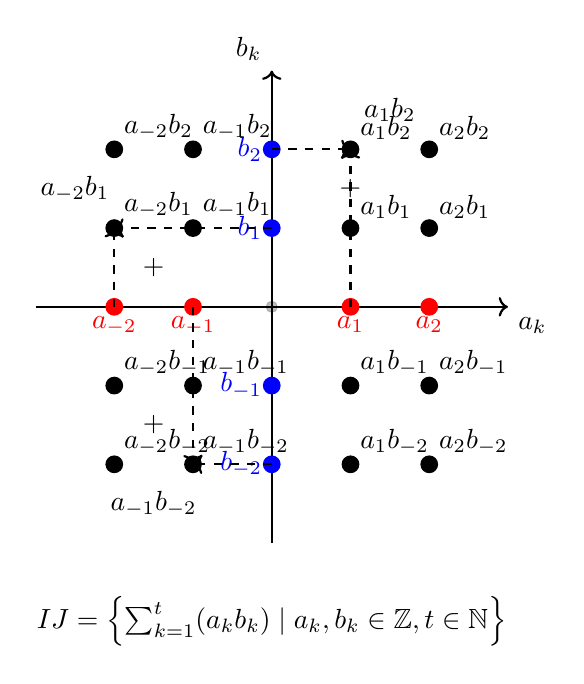
\begin{tikzpicture}[scale=1.0]

% Define the grid
\foreach \x in {-2, -1, 0, 1, 2}
{
	\foreach \y in {-2, -1, 0, 1, 2}
	{
		\filldraw[gray,opacity=0.5] (\x,\y) circle (2pt);
	}
}

% Axes
\draw[thick,->] (-3,0) -- (3,0) node[anchor=north west] {$a_k$};
\draw[thick,->] (0,-3) -- (0,3) node[anchor=south east] {$b_k$};

% Points for I = (a)
\foreach \x in {-2, -1, 1, 2}
{
	\filldraw[red] (\x,0) circle (3pt);
	\node[red, below] at (\x, 0) {$a_{\x}$};
}

% Points for J = (b)
\foreach \y in {-2, -1, 1, 2}
{
	\filldraw[blue] (0,\y) circle (3pt);
	\node[blue, left] at (0, \y) {$b_{\y}$};
}

% Points for Product a_i * b_j
\foreach \x in {-2, -1, 1, 2}
{
	\foreach \y in {-2, -1, 1, 2}
	{
		\filldraw[black] (\x,\y) circle (3pt);
		\node[black, above right] at (\x, \y) {$a_{\x}b_{\y}$};
	}
}

% Summation example
\draw[thick, ->, dashed] (1, 0) -- (1, 2);
\draw[thick, ->, dashed] (0, 2) -- (1, 2);
\node[align=left] at (1, 1.5) {$+$};
\node[align=left] at (1.5, 2.5) {$a_1 b_2$};

\draw[thick, ->, dashed] (-2, 0) -- (-2, 1);
\draw[thick, ->, dashed] (0, 1) -- (-2, 1);
\node[align=left] at (-1.5, 0.5) {$+$};
\node[align=left] at (-2.5, 1.5) {$a_{-2} b_1$};

\draw[thick, ->, dashed] (-1, 0) -- (-1, -2);
\draw[thick, ->, dashed] (0, -2) -- (-1, -2);
\node[align=left] at (-1.5, -1.5) {$+$};
\node[align=left] at (-1.5, -2.5) {$a_{-1} b_{-2}$};

% Summation label
\node[align=center] at (0, -4) {$IJ = \left\{\sum_{k=1}^{t}(a_k b_k) \mid a_k, b_k \in \mathbb{Z}, t \in \mathbb{N} \right\}$};

\end{tikzpicture}
\[
\Z\Z=\set{\sum_{k=1}^{t}(a_k)(b_k):a_k,b_k\in\Z,t\in\N}
\]



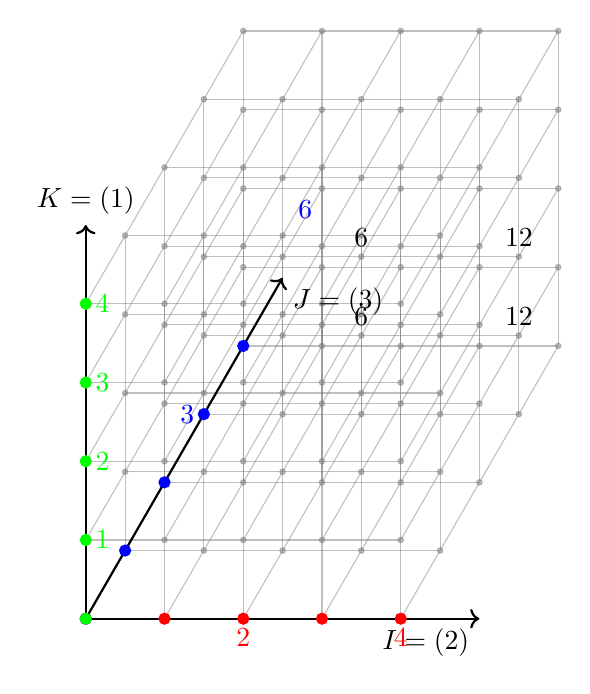
\begin{tikzpicture}[scale=1.0, x={(1cm,0cm)}, y={(0.5cm,0.866cm)}, z={(0cm,1cm)}]

% Define the size of the grid
\def\xmax{4}
\def\ymax{4}
\def\zmax{4}

% Draw the 3D grid
\foreach \x in {0,...,\xmax}
{
	\foreach \y in {0,...,\ymax}
	{
		\foreach \z in {0,...,\zmax}
		{
			\filldraw[gray,opacity=0.5] (\x,\y,\z) circle (1pt);
		}
	}
}

% Draw the grid lines parallel to the x-axis
\foreach \y in {0,...,\ymax}
{
	\foreach \z in {0,...,\zmax}
	{
		\draw[gray,opacity=0.5] (0,\y,\z) -- (\xmax,\y,\z);
	}
}

% Draw the grid lines parallel to the y-axis
\foreach \x in {0,...,\xmax}
{
	\foreach \z in {0,...,\zmax}
	{
		\draw[gray,opacity=0.5] (\x,0,\z) -- (\x,\ymax,\z);
	}
}

% Draw the grid lines parallel to the z-axis
\foreach \x in {0,...,\xmax}
{
	\foreach \y in {0,...,\ymax}
	{
		\draw[gray,opacity=0.5] (\x,\y,0) -- (\x,\y,\zmax);
	}
}

% Draw the axes
\draw[thick,->] (0,0,0) -- (5,0,0) node[anchor=north east] {$I = (2)$};
\draw[thick,->] (0,0,0) -- (0,5,0) node[anchor=north west] {$J = (3)$};
\draw[thick,->] (0,0,0) -- (0,0,5) node[anchor=south] {$K = (1)$};

% Points for Ideal I (multiples of 2)
\foreach \x in {0,1,2,3,4}
{
	\filldraw[red] (\x,0,0) circle (2pt);
}

% Points for Ideal J (multiples of 3)
\foreach \y in {0,1,2,3,4}
{
	\filldraw[blue] (0,\y,0) circle (2pt);
}

% Points for Ideal K (multiples of 1)
\foreach \z in {0,1,2,3,4}
{
	\filldraw[green] (0,0,\z) circle (2pt);
}

% Points for Product Ideal IJ = (6)
%		\foreach \x in {0,1,2,3,4}
%		{
	%			\foreach \y in {0,1,2,3,4}
	%			{
		%				\foreach \z in {0,1,2,3,4}
		%				{
			%					\ifnum \numexpr \x*\y*\z = \numexpr \x*\y*\z/6*6
			%					\filldraw[black] (\x,\y,\z) circle (2pt);
			%					\fi
			%				}
		%			}
	%		}

% Labels
\node[red, below] at (2, 0, 0) {$2$};
\node[red, below] at (4, 0, 0) {$4$};

\node[blue, left] at (0, 3, 0) {$3$};
\node[blue, left] at (0, 6, 0) {$6$};

\node[green, right] at (0, 0, 1) {$1$};
\node[green, right] at (0, 0, 2) {$2$};
\node[green, right] at (0, 0, 3) {$3$};
\node[green, right] at (0, 0, 4) {$4$};

\node[black, above] at (2, 3, 1) {$6$};
\node[black, above] at (2, 3, 2) {$6$};
\node[black, above] at (4, 3, 1) {$12$};
\node[black, above] at (4, 3, 2) {$12$};

\end{tikzpicture}
\newpage
\adjustbox{scale=.7}{
\begin{tabular}{|>{\centering\arraybackslash}m{4cm}|>{\centering\arraybackslash}m{3cm}|>{\centering\arraybackslash}m{3cm}|>{\centering\arraybackslash}m{1.5cm}|>{\centering\arraybackslash}m{1.5cm}|>{\centering\arraybackslash}m{2cm}|>{\centering\arraybackslash}m{2cm}|}
	\hline
	\textbf{Ring (Set)} & \textbf{Addition Operation} & \textbf{Multiplication Operation} & \textbf{Additive Identity} & \textbf{Multiplicative Identity} & \textbf{Form of Element} & \textbf{Commutative} \\
	\hline
	Integers \( \mathbb{Z} \) & Standard addition \( + \) & Standard multiplication \( \cdot \) & \( 0 \) & \( 1 \) & Integers & Yes \\
	\hline
	Real Numbers \( \mathbb{R} \) & Standard addition \( + \) & Standard multiplication \( \cdot \) & \( 0 \) & \( 1 \) & Real numbers & Yes \\
	\hline
	Complex Numbers \( \mathbb{C} \) & Standard addition \( + \) & Standard multiplication \( \cdot \) & \( 0 \) & \( 1 \) & \( a + bi \) where \( a, b \in \mathbb{R} \) & Yes \\
	\hline
	Polynomials with Real Coefficients \( \mathbb{R}[x] \) & Polynomial addition & Polynomial multiplication & \( 0 \) (zero polynomial) & \( 1 \) (constant polynomial) & \( a_n x^n + \cdots + a_1 x + a_0 \) & Yes \\
	\hline
	Matrices \( M_n(\mathbb{R}) \) & Matrix addition & Matrix multiplication & Zero matrix & Identity matrix & \( n \times n \) matrices & No \\
	\hline
	Integers Modulo \( n \) \( \mathbb{Z}/n\mathbb{Z} \) & Addition modulo \( n \) & Multiplication modulo \( n \) & \( 0 \) & \( 1 \) & \( \{ 0, 1, \ldots, n-1 \} \) & Yes \\
	\hline
\end{tabular}}
\begin{center}
\begin{tabular}{|>{\centering\arraybackslash}m{3cm}|>{\centering\arraybackslash}m{2cm}|>{\centering\arraybackslash}m{1.5cm}|>{\centering\arraybackslash}m{4cm}|>{\centering\arraybackslash}m{4cm}|>{\centering\arraybackslash}m{1.5cm}|}
	\hline
	\textbf{Group (Set)} & \textbf{Operation} & \textbf{Identity} & \textbf{Form of Element} & \textbf{Normal Subgroups} & \textbf{Abelian} \\
	\hline
	Symmetric Group \( S_3 \) & Composition of permutations & Identity permutation \( e \) & Permutations of 3 elements & \(\{ e, (123), (132) \}\), \(\{ e, (12), (13), (23), (123), (132) \}\) & No \\
	\hline
	Dihedral Group \( D_4 \) & Composition of symmetries & Identity symmetry \( e \) & Rotations \( r^k \) and reflections \( sr^k \), \( k \in \{0, 1, 2, 3\} \) & \(\{ e, r, r^2, r^3 \}\), \(\{ e, r^2, s, sr^2 \}\) & No \\
	\hline
	Quaternion Group \( Q_8 \) & Quaternion multiplication & \( 1 \) & Quaternions \( \pm 1, \pm i, \pm j, \pm k \) & \(\{ 1, -1 \}\), \(\{ 1, -1, i, -i \}\), \(\{ 1, -1, j, -j \}\), \(\{ 1, -1, k, -k \}\) & No \\
	\hline
	Integers Modulo \( n \) \( \mathbb{Z}/n\mathbb{Z} \) & Addition modulo \( n \) & \( 0 \) & \( \{0, 1, \ldots, n-1\} \) & All subgroups are normal & Yes \\
	\hline
\end{tabular}
\end{center}
\adjustbox{scale=.5}{
\begin{tabular}{ccccccc}
	\hline
	\textbf{Ring (Set)} & \textbf{Addition Operation} & \textbf{Multiplication Operation} & \textbf{Additive Identity} & \textbf{Multiplicative Identity} & \textbf{Form of Element} \\
	\hline
	Matrices \( M_n(\mathbb{R}) \) & Matrix addition & Matrix multiplication & Zero matrix & Identity matrix & \( n \times n \) matrices \\
	\hline
	Quaternions \( \mathbb{H} \) & Quaternion addition & Quaternion multiplication & \( 0 \) & \( 1 \) & \( a + bi + cj + dk \) where \( a, b, c, d \in \mathbb{R} \) \\
	\hline
	Differential Operators & Operator addition & Operator composition & Zero operator & Identity operator & \( \sum a_i \frac{d^i}{dx^i} \) \\
	\hline
	Group Rings \( \mathbb{R}[G] \) & Group ring addition & Group ring multiplication & Zero element & Identity element & \( \sum a_g g \) where \( a_g \in \mathbb{R} \) and \( g \in G \) \\
	\hline
	Endomorphism Rings \( \text{End}(V) \) & Function addition & Function composition & Zero map & Identity map & Linear transformations on vector space \( V \) \\
	\hline
	Octonions \( \mathbb{O} \) & Octonion addition & Octonion multiplication & \( 0 \) & \( 1 \) & \( a + b e_1 + c e_2 + d e_3 + e e_4 + f e_5 + g e_6 + h e_7 \) where \( a, b, c, d, e, f, g, h \in \mathbb{R} \) \\
	\hline
\end{tabular}}
\begin{center}
\begin{tabular}{|>{\centering\arraybackslash}m{4cm}|>{\centering\arraybackslash}m{2cm}|>{\centering\arraybackslash}m{2cm}|>{\centering\arraybackslash}m{2cm}|>{\centering\arraybackslash}m{2cm}|}
	\hline
	\textbf{Type} & \textbf{Ideal} & \textbf{Principal Ideal} & \textbf{Prime Ideal} & \textbf{Maximal Ideal} \\
	\hline
	\textbf{Definition} & A subset closed under addition and multiplication by any ring element & An ideal generated by a single element & An ideal where if \(ab \in I\), then \(a \in I\) or \(b \in I\) & An ideal such that there are no larger ideals except the ring itself \\
	\hline
	Is an Ideal & \(O\) & \(O\) & \(O\) & \(O\) \\
	\hline
	Can be Principal & \(O\) & \(O\) & \(O\) & \(O\) \\
	\hline
	Is Prime & \(X\) & \(X\) & \(O\) & \(O\) \\
	\hline
	Is Maximal & \(X\) & \(X\) & \(X\) & \(O\) \\
	\hline
\end{tabular}
\end{center}

\begin{center}
\begin{tabular}{|>{\centering\arraybackslash}m{4cm}|>{\centering\arraybackslash}m{3cm}|>{\centering\arraybackslash}m{3cm}|>{\centering\arraybackslash}m{3cm}|}
	\hline
	\textbf{Ring (Set)} & \textbf{Principal Ideals} & \textbf{Prime Ideals} & \textbf{Maximal Ideals} \\
	\hline
	\(\mathbb{Z}\) & \((2), (3), (5)\) & \((2), (3), (5)\) & \((2), (3), (5)\) \\
	\hline
	\(\mathbb{R}[x]\) & \((x), (x-1), (x^2+1)\) & \((x)\) & \((x-1)\) \\
	\hline
	\(\mathbb{C}[x]\) & \((x), (x-i), (x+i)\) & \((x-i), (x+i)\) & \((x-i), (x+i)\) \\
	\hline
	\(\mathbb{Z}/6\mathbb{Z}\) & \((2), (3)\) & None & \((2), (3)\) \\
	\hline
	\(\mathbb{Z}[i]\) & \((1+i), (2)\) & \((1+i)\) & \((1+i)\) \\
	\hline
	\(\mathbb{Z}/p\mathbb{Z}\) where \(p\) is prime & \((0), (1)\) & \((0)\) & \((0)\) \\
	\hline
	\(\mathbb{R}\) & \((0)\) & None & \((0)\) \\
	\hline
	\(\mathbb{C}\) & \((0)\) & None & \((0)\) \\
	\hline
	\(\mathbb{Z}[x]\) & \((2), (3), (x)\) & \((x), (2)\) & None \\
	\hline
	\(M_n(\mathbb{R})\) & \((E_{11})\) & None & None \\
	\hline
	\(\mathbb{H}\) (Quaternions) & \((1+i)\) & None & None \\
	\hline
\end{tabular}
\end{center}

\begin{center}
\begin{tabular}{|>{\centering\arraybackslash}m{4cm}|>{\centering\arraybackslash}m{4cm}|>{\centering\arraybackslash}m{4cm}|>{\centering\arraybackslash}m{4cm}|}
	\hline
	\textbf{Ring (Set)} & \textbf{Principal Ideals} & \textbf{Prime Ideals} & \textbf{Maximal Ideals} \\
	\hline
	\(\mathbb{Z}\) & \((2) = \{2k \mid k \in \mathbb{Z}\}\) & \((2) = \{2k \mid k \in \mathbb{Z}\}\) & \((2) = \{2k \mid k \in \mathbb{Z}\}\) \\
	& \((3) = \{3k \mid k \in \mathbb{Z}\}\) & \((3) = \{3k \mid k \in \mathbb{Z}\}\) & \((3) = \{3k \mid k \in \mathbb{Z}\}\) \\
	& \((5) = \{5k \mid k \in \mathbb{Z}\}\) & \((5) = \{5k \mid k \in \mathbb{Z}\}\) & \((5) = \{5k \mid k \in \mathbb{Z}\}\) \\
	\hline
	\(\mathbb{R}[x]\) & \((x) = \{x f(x) \mid f(x) \in \mathbb{R}[x]\}\) & \((x) = \{x f(x) \mid f(x) \in \mathbb{R}[x]\}\) & \((x-1) = \{(x-1) f(x) \mid f(x) \in \mathbb{R}[x]\}\) \\
	& \((x-1) = \{(x-1) f(x) \mid f(x) \in \mathbb{R}[x]\}\) &  &  \\
	& \((x^2+1) = \{(x^2+1) f(x) \mid f(x) \in \mathbb{R}[x]\}\) &  &  \\
	\hline
	\(\mathbb{C}[x]\) & \((x) = \{x f(x) \mid f(x) \in \mathbb{C}[x]\}\) & \((x-i) = \{(x-i) f(x) \mid f(x) \in \mathbb{C}[x]\}\) & \((x-i) = \{(x-i) f(x) \mid f(x) \in \mathbb{C}[x]\}\) \\
	& \((x-i) = \{(x-i) f(x) \mid f(x) \in \mathbb{C}[x]\}\) & \((x+i) = \{(x+i) f(x) \mid f(x) \in \mathbb{C}[x]\}\) & \((x+i) = \{(x+i) f(x) \mid f(x) \in \mathbb{C}[x]\}\) \\
	& \((x+i) = \{(x+i) f(x) \mid f(x) \in \mathbb{C}[x]\}\) &  &  \\
	\hline
	\(\mathbb{Z}/6\mathbb{Z}\) & \((2) = \{0, 2, 4\}\) & None & \((2) = \{0, 2, 4\}\) \\
	& \((3) = \{0, 3\}\) &  & \((3) = \{0, 3\}\) \\
	\hline
	\(\mathbb{Z}[i]\) & \((1+i) = \{(1+i) z \mid z \in \mathbb{Z}[i]\}\) & \((1+i) = \{(1+i) z \mid z \in \mathbb{Z}[i]\}\) & \((1+i) = \{(1+i) z \mid z \in \mathbb{Z}[i]\}\) \\
	& \((2) = \{2 z \mid z \in \mathbb{Z}[i]\}\) &  &  \\
	\hline
	\(\mathbb{Z}/p\mathbb{Z}\) where \(p\) is prime & \((0) = \{0\}\) & \((0) = \{0\}\) & \((0) = \{0\}\) \\
	& \((1) = \mathbb{Z}/p\mathbb{Z}\) &  &  \\
	\hline
	\(\mathbb{R}\) & \((0) = \{0\}\) & None & \((0) = \{0\}\) \\
	\hline
	\(\mathbb{C}\) & \((0) = \{0\}\) & None & \((0) = \{0\}\) \\
	\hline
	\(\mathbb{Z}[x]\) & \((2) = \{2 f(x) \mid f(x) \in \mathbb{Z}[x]\}\) & \((2) = \{2 f(x) \mid f(x) \in \mathbb{Z}[x]\}\) & None \\
	& \((3) = \{3 f(x) \mid f(x) \in \mathbb{Z}[x]\}\) &  &  \\
	& \((x) = \{x f(x) \mid f(x) \in \mathbb{Z}[x]\}\) & \((x) = \{x f(x) \mid f(x) \in \mathbb{Z}[x]\}\) &  \\
	\hline
	\(M_n(\mathbb{R})\) & \((E_{11}) = \{A E_{11} B \mid A, B \in M_n(\mathbb{R})\}\) & None & None \\
	\hline
	\(\mathbb{H}\) (Quaternions) & \((1+i) = \{(1+i) q \mid q \in \mathbb{H}\}\) & None & None \\
	\hline
\end{tabular}
\end{center}

\begin{center}
\begin{tabular}{|>{\centering\arraybackslash}m{4cm}|>{\centering\arraybackslash}m{4cm}|>{\centering\arraybackslash}m{4cm}|>{\centering\arraybackslash}m{4cm}|}
	\hline
	\textbf{Ring (Set)} & \textbf{Principal Ideals} & \textbf{Prime Ideals} & \textbf{Maximal Ideals} \\
	\hline
	\(\mathbb{Z}\) & \((2) = \{2k \mid k \in \mathbb{Z}\}\) & \((2) = \{2k \mid k \in \mathbb{Z}\}\) & \((2) = \{2k \mid k \in \mathbb{Z}\}\) \\
	& \((3) = \{3k \mid k \in \mathbb{Z}\}\) & \((3) = \{3k \mid k \in \mathbb{Z}\}\) & \((3) = \{3k \mid k \in \mathbb{Z}\}\) \\
	& \((5) = \{5k \mid k \in \mathbb{Z}\}\) & \((5) = \{5k \mid k \in \mathbb{Z}\}\) & \((5) = \{5k \mid k \in \mathbb{Z}\}\) \\
	\hline
	\(\mathbb{R}[x]\) & \((x) = \{x f(x) \mid f(x) \in \mathbb{R}[x]\}\) & \((x)\) & \((x-1)\) \\
	& \((x-1) = \{(x-1) f(x) \mid f(x) \in \mathbb{R}[x]\}\) &  &  \\
	& \((x^2+1) = \{(x^2+1) f(x) \mid f(x) \in \mathbb{R}[x]\}\) &  &  \\
	\hline
	\(\mathbb{C}[x]\) & \((x) = \{x f(x) \mid f(x) \in \mathbb{C}[x]\}\) & \((x-i)\) & \((x-i)\) \\
	& \((x-i) = \{(x-i) f(x) \mid f(x) \in \mathbb{C}[x]\}\) & \((x+i)\) & \((x+i)\) \\
	& \((x+i) = \{(x+i) f(x) \mid f(x) \in \mathbb{C}[x]\}\) &  &  \\
	\hline
	\(\mathbb{Z}/6\mathbb{Z}\) & \((2) = \{0, 2, 4\}\) & None & \((2) = \{0, 2, 4\}\) \\
	& \((3) = \{0, 3\}\) &  & \((3) = \{0, 3\}\) \\
	\hline
	\(\mathbb{Z}[i]\) & \((1+i) = \{(1+i) z \mid z \in \mathbb{Z}[i]\}\) & \((1+i)\) & \((1+i)\) \\
	& \((2) = \{2 z \mid z \in \mathbb{Z}[i]\}\) &  &  \\
	\hline
	\(\mathbb{Z}/p\mathbb{Z}\) where \(p\) is prime & \((0) = \{0\}\) & \((0)\) & \((0)\) \\
	& \((1) = \mathbb{Z}/p\mathbb{Z}\) &  &  \\
	\hline
	\(\mathbb{R}\) & \((0) = \{0\}\) & None & \((0)\) \\
	\hline
	\(\mathbb{C}\) & \((0) = \{0\}\) & None & \((0)\) \\
	\hline
	\(\mathbb{Z}[x]\) & \((2) = \{2 f(x) \mid f(x) \in \mathbb{Z}[x]\}\) & \((2)\) & None \\
	& \((3) = \{3 f(x) \mid f(x) \in \mathbb{Z}[x]\}\) &  &  \\
	& \((x) = \{x f(x) \mid f(x) \in \mathbb{Z}[x]\}\) & \((x)\) &  \\
	\hline
	\(M_n(\mathbb{R})\) & \((E_{11}) = \{A E_{11} B \mid A, B \in M_n(\mathbb{R})\}\) & None & None \\
	\hline
	\(\mathbb{H}\) (Quaternions) & \((1+i) = \{(1+i) q \mid q \in \mathbb{H}\}\) & None & None \\
	\hline
\end{tabular}
\end{center}

\newpage
\adjustbox{scale=.7}{
\begin{tabular}{|ccccc|}
	\hline
	\textbf{Ring (Set)} & \textbf{Examples of Ideals} & \textbf{Examples of Principal Ideals} & \textbf{Examples of Prime Ideals} & \textbf{Examples of Maximal Ideals} \\
	\hline
	\(\mathbb{Z}\) & \((0), (2), (3)\) & \((2) = \{2k \mid k \in \mathbb{Z}\}\) & \((2) = \{2k \mid k \in \mathbb{Z}\}\) & \((2) = \{2k \mid k \in \mathbb{Z}\}\) \\
	& \((4), (6)\) & \((3) = \{3k \mid k \in \mathbb{Z}\}\) & \((3) = \{3k \mid k \in \mathbb{Z}\}\) & \((3) = \{3k \mid k \in \mathbb{Z}\}\) \\
	& \((0)\) & \((5) = \{5k \mid k \in \mathbb{Z}\}\) & \((5) = \{5k \mid k \in \mathbb{Z}\}\) & \((5) = \{5k \mid k \in \mathbb{Z}\}\) \\
	\hline
	\(\mathbb{R}[x]\) & \((0), (x), (x-1)\) & \((x) = \{x f(x) \mid f(x) \in \mathbb{R}[x]\}\) & \((x)\) & \((x-1)\) \\
	& \((x^2+1)\) & \((x-1) = \{(x-1) f(x) \mid f(x) \in \mathbb{R}[x]\}\) &  &  \\
	&  & \((x^2+1) = \{(x^2+1) f(x) \mid f(x) \in \mathbb{R}[x]\}\) &  &  \\
	\hline
	\(\mathbb{C}[x]\) & \((0), (x), (x-i)\) & \((x) = \{x f(x) \mid f(x) \in \mathbb{C}[x]\}\) & \((x-i)\) & \((x-i)\) \\
	& \((x+i)\) & \((x-i) = \{(x-i) f(x) \mid f(x) \in \mathbb{C}[x]\}\) & \((x+i)\) & \((x+i)\) \\
	&  & \((x+i) = \{(x+i) f(x) \mid f(x) \in \mathbb{C}[x]\}\) &  &  \\
	\hline
	\(\mathbb{Z}/6\mathbb{Z}\) & \((0), (2), (3)\) & \((2) = \{0, 2, 4\}\) & None & \((2) = \{0, 2, 4\}\) \\
	&  & \((3) = \{0, 3\}\) &  & \((3) = \{0, 3\}\) \\
	\hline
	\(\mathbb{Z}[i]\) & \((0), (1+i), (2)\) & \((1+i) = \{(1+i) z \mid z \in \mathbb{Z}[i]\}\) & \((1+i)\) & \((1+i)\) \\
	&  & \((2) = \{2 z \mid z \in \mathbb{Z}[i]\}\) &  &  \\
	\hline
	\(\mathbb{Z}/p\mathbb{Z}\) where \(p\) is prime & \((0), (1)\) & \((0) = \{0\}\) & \((0)\) & \((0)\) \\
	&  & \((1) = \mathbb{Z}/p\mathbb{Z}\) &  &  \\
	\hline
	\(\mathbb{R}\) & \((0)\) & \((0) = \{0\}\) & None & \((0)\) \\
	\hline
	\(\mathbb{C}\) & \((0)\) & \((0) = \{0\}\) & None & \((0)\) \\
	\hline
	\(\mathbb{Z}[x]\) & \((0), (2), (3)\) & \((2) = \{2 f(x) \mid f(x) \in \mathbb{Z}[x]\}\) & \((2)\) & None \\
	&  & \((3) = \{3 f(x) \mid f(x) \in \mathbb{Z}[x]\}\) &  &  \\
	&  & \((x) = \{x f(x) \mid f(x) \in \mathbb{Z}[x]\}\) & \((x)\) &  \\
	\hline
	\(M_n(\mathbb{R})\) & \((0), (E_{11})\) & \((E_{11}) = \{A E_{11} B \mid A, B \in M_n(\mathbb{R})\}\) & None & None \\
	\hline
	\(\mathbb{H}\) (Quaternions) & \((0), (1+i)\) & \((1+i) = \{(1+i) q \mid q \in \mathbb{H}\}\) & None & None \\
	\hline
\end{tabular}}
\end{document}
